\documentclass[12pt,letterpaper,oneside,titlepage]{book}
\usepackage[margin=1in]{geometry}
\usepackage{indentfirst}
\usepackage{enumitem}

\usepackage[utf8]{inputenc}
\usepackage[T2A]{fontenc}
\usepackage{textcomp}

\usepackage{xspace}
% \usepackage{xcolor}
\usepackage{tikz}

\usepackage[
  hyperfootnotes=false,
  hidelinks,
  linktoc=all,
  pdfauthor={Ivan Pogrebnyak},
  pdftitle={Brewing notes}
]{hyperref}

\author{Ivan Pogrebnyak}
\title{Brewing Notes}
\date{\today}

\setcounter{secnumdepth}{-1}
\setcounter{tocdepth}{1}
% \renewcommand{\thechapter}{}
% \renewcommand{\chaptername}{}
% \makeatletter
% \renewcommand{\thesection}{\arabic{section}}
% \makeatother

\newcommand{\degC}{°C\xspace}
\newcommand{\x}{×\xspace}

\begin{document}

\frontmatter

\begin{titlepage}
  \tikz[remember picture,overlay]
  \node[opacity=0.3,inner sep=0pt,xshift=0.30in]
    at (current page.center){
    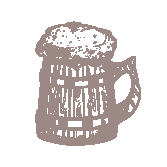
\includegraphics[width=1.1\paperwidth]{fig/mug.pdf}
  };
  \makeatletter
  \vspace{3.31in}
  \begin{center}
    {\Huge\textbf{\@title}}\\[0.25in]
    \vspace{2.4in}
    \@author\\\@date
  \end{center}
  \makeatother
\end{titlepage}

\setcounter{page}{2}
\tableofcontents

% \setlength{\parindent}{0pt}
\setlength{\parskip}{0.25em}

%%%%%%%%%%%%%%%%%%%%%%%%%%%%%%%%%%%%%%%%%%%%%%%%%%%%%%%%%%%%%%%%%%%%%

\mainmatter
\chapter{Notes}

\section{Priming}
Boil 1 cup of white sugar in 1 pint of water for 5 gallons of beer.

\section{Fermentation}
The optimal temperature of fermentation for ale yeast is 15--24 \degC.

Secondary fermentation is not needed for any beer that ferments for
2 weeks or less.
Ales can be fermented in one go.
For lagers, transferring to a secondary fermenter serves to remove dead yeast,
which can negatively impact the flavor when they start to break down.

%%%%%%%%%%%%%%%%%%%%%%%%%%%%%%%%%%%%%%%%%%%%%%%%%%%%%%%%%%%%%%%%%%%%%

\makeatletter
\renewcommand{\section}{\@startsection
{section}%                   % the name
{1}%                         % the level
{0mm}%                       % the indent
{-\baselineskip}%            % the before skip
{0.5\baselineskip}%          % the after skip
{\hspace{-\parindent}%

\includegraphics[width=1.2em]{fig/mug-icon.pdf}%
~~\bfseries\Large}} % the style
\makeatother

\chapter{Recipes}
\section{Lavender Dew}
A pale ale with floral aroma.

\subsection{Ingredients}
For 5 gallons of beer:
\begin{itemize}[noitemsep]
  \item Light malt extract: 6 lb, liquid
  \item Wild flower honey: 1 lb
  \item Yeast: SafAle™ US-05
  \item Hops: Goldings, 2 \x 1 oz bags, pellets
  \item Lavender: 1.5 tbsp
  \item Coriander: 2 tbsp, crushed whole
  \item Chamomile: 3 tbsp
  \item Heather tips: 1.5 tbsp
  \item Ginger: 3 tbsp
\end{itemize}

\subsection{Instructions}

Boil malt extract and honey for a few minutes until fully dissolved.

Add hops in 3 batches:
first 1 oz, 20 minutes later 0.5 oz, 8 minutes later 0.5 oz.
Continue boiling the wart for another 2 minutes.
Add all herbs with the first batch of hops.

\end{document}
